\section{Introduction}

Recovering contact geometry from touch gives a robot information about where an object meets its fingertip and how the object is oriented. Vision-based tactile sensors obtain this information by imaging the deformation of a soft elastomer. GelSight, GelSlim and DIGIT~\cite{yuan2017gelsight,donlon2018gelslim,lambeta2020digit} follow this principle, but their images differ with illumination, elastomer properties and camera response. Learning a geometric predictor requires examples of the target sensor's appearance together with accurate labels. We consider known-object perception: object identity and a mesh are available, but registering every captured contact to that mesh is costly.

\begin{figure*}[t]
    \centering
    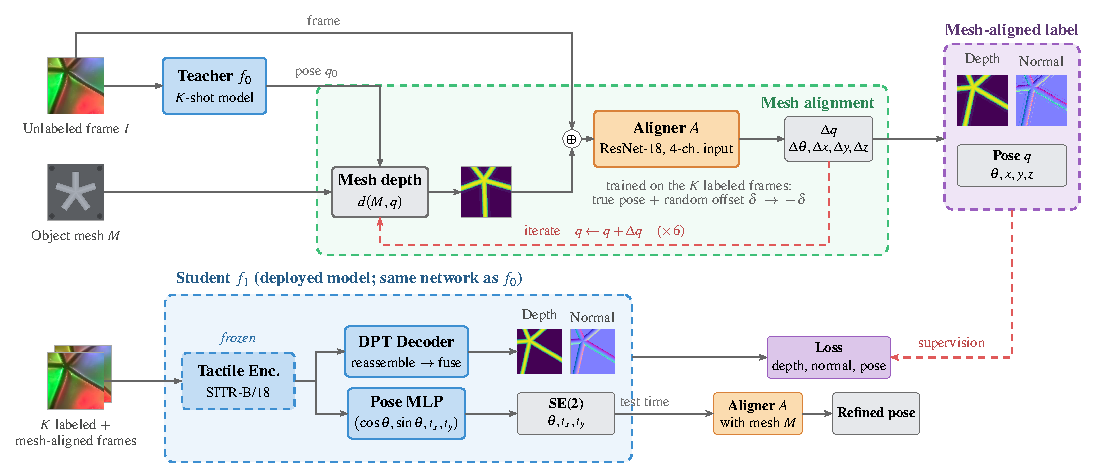
\includegraphics[width=0.97\textwidth]{figures/fig_arch.pdf}
    \caption{\textbf{Overview of MeshTac.} Teacher $f_0$ initializes the contact state. Aligner $A$ compares the frame with mesh depth and predicts a correction, applied six times. The aligned mesh supplies depth, normal and planar-pose targets for student $f_1$, which shares the teacher's architecture. All components use the same $K$ real training labels; the main sensor-A pipeline also uses synthetic examples, omitted here. The student requires no mesh at inference; optional pose refinement uses the image, mesh and fixed aligner. Blue: perception networks; orange: aligner; grey: geometry and pose; purple: labels and loss. Thumbnails show a $K=25$ example, including the student's actual prediction.}
    \label{fig:mapl}
\end{figure*}

Simulation can reduce the need for registered real contacts by generating tactile images and geometric labels from known meshes~\cite{wang2022tacto,si2022taxim,chen2023tacchi}. Its usefulness depends on whether the rendered appearance supports learning on the real sensor. Learned renderers can improve this correspondence, but training them also consumes real labels. A fair assessment of label efficiency must therefore count the supervision used by both the renderer and the downstream model.

Our renderer study exposes the importance of this accounting. A model augmented with images from a renderer trained on all real training pairs appears substantially more accurate than a model trained on a small labeled subset. Much of this advantage disappears when both components are restricted to the same subset: in the few-label regime on sensor A, learned rendering slightly lowers all-pixel depth error while worsening contact error and overlap. This finding motivates a more direct use of the mesh to supervise real images.

An unlabeled tactile image already contains the target sensor's appearance. If the object mesh is known, the missing information for a geometric label is its contact state: in-plane rotation, translation and indentation. A model trained on a small labeled set can initialize this state. Its estimate is often too imprecise to use directly, however, because pose errors shift the projected contact and corrupt the resulting dense labels. The central challenge is to align the mesh accurately enough for the additional images to become useful training data.

MeshTac addresses this challenge with a learned residual aligner (Fig.~\ref{fig:mapl}). Given a real image and mesh depth at a candidate state, the aligner predicts a correction. Perturbing the registered contacts supplies training examples without additional real labels. Unlike refinement used only at inference, MeshTac converts each corrected state into depth, normal and pose targets for training on real images. The student retains real contact appearance during training and predicts without a mesh at standard inference.

We evaluate MeshTac against real-only training, synthetic-data augmentation and teacher-based self-training under matched training-label budgets. Experiments with models trained separately for each sensor show that alignment improves both pseudo-label quality and the student's contact reconstruction. Renderer-free and second-session experiments distinguish the contribution of geometric supervision from that of synthetic appearance. Our contributions are:
\begin{itemize}
    \item \textbf{Mesh-aligned pseudo-labeling for known-object tactile perception.} MeshTac learns contact-state refinement from a small registered set and converts the refined meshes into consistent depth, normal and pose targets for unlabeled real images; the trained student remains mesh-free at standard inference.
    \item \textbf{Label accounting for tactile simulation.} A controlled study gives the renderer and downstream model the same real training-label budget, separating gains from synthetic data from gains obtained with additional paired real contacts.
    \item \textbf{Systematic empirical characterization.} Experiments with separately trained models on two sensors, a second capture session and held-out objects isolate the roles of alignment and synthetic data; they also evaluate reuse of the same aligner for optional test-time pose refinement without retraining.
\end{itemize}
